% https://tex.stackexchange.com/questions/180888/tikz-extend-a-line-along-a-path
\documentclass[tikz]{standalone}

\usetikzlibrary{decorations.markings}

\begin{document}
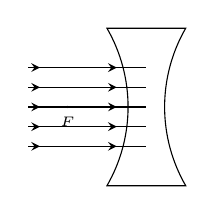
\begin{tikzpicture}
  \pgfmathsetmacro{\lH}{1}
  \pgfmathsetmacro{\lR}{2}
  \pgfmathsetmacro{\sA}{asin(\lH/\lR)}
  \pgfmathsetmacro{\base}{1}
  \pgfmathsetmacro{\xshi}{\base/2}

  \draw[yshift = -2cm, xshift = -\xshi cm] (0, \lH cm)
  arc[start angle = -\sA, delta angle = 2*\sA, radius = \lR cm] --
  +(\base cm, 0)
  arc[start angle = 180 - \sA, delta angle = 2*\sA, radius = \lR cm]
   -- cycle;

  \begin{scope}[decoration = {
      markings,
      mark = at position 0.1 with {\arrow{stealth}},
      mark = at position 0.75 with {\arrow{stealth}}
    }
    ]
    \foreach \y in {0.5, 0.25, 0, -0.25, -0.5}{
      \draw[postaction = decorate] (-1.5cm, \y cm) -- (0, \y cm); %extend lines along the path command here;
    }
  \end{scope}

  \fill[fill = black] (-1cm, 0) circle[radius = 0.015cm] node[below,
  font = \tiny] {$F$}; 
\end{tikzpicture}
\end{document}

%%% Local Variables:
%%% mode: latex
%%% TeX-master: t
%%% End:
